\documentclass[a4paper,12pt]{article}

\usepackage{cmap}					% поиск в PDF
\usepackage[utf8]{inputenc}
\usepackage[T2A]{fontenc}
\usepackage[english,russian]{babel}
\usepackage[autostyle]{csquotes}
\usepackage{graphicx}
\usepackage{caption}
\usepackage{listings}
\usepackage{float}
\usepackage[authoryear,round]{natbib}
\usepackage{biblatex}
\graphicspath{ {images/} }
\author{Казакова Элиза}
\date{\today}
\usepackage[left=2cm,right=2cm,top=2cm,bottom=2cm,bindingoffset=0cm]{geometry}
\newcommand{\anonsection}[1]{\section*{#1}\addcontentsline{toc}{section}{#1}}
\begin{document} % Конец преамбулы, начало текста.
	
\begin{titlepage}
	\fontsize{12pt}{12pt}\selectfont
	\noindent \begin{minipage}{0.15\textwidth}
		
\includegraphics[width=\linewidth]{ MGTU.png}
	\end{minipage}
	\noindent\begin{minipage}{0.9\textwidth}\centering
		\textbf{Министерство науки и высшего образования Российской Федерации}\\
		\textbf{Федеральное государственное бюджетное образовательное учреждение высшего образования}\\
		\textbf{«Московский государственный технический университет имени Н.Э.~Баумана}\\
		\textbf{(национальный исследовательский университет)»}\\
		\textbf{(МГТУ им. Н.Э.~Баумана)}
	\end{minipage}
	
	\noindent\rule{18cm}{3pt}
	\newline\newline
	\noindent 
	ФАКУЛЬТЕТ 
	\underline{«Информатика и системы управления»} \newline\newline
	
	\noindent КАФЕДРА \underline{«Программное обеспечение ЭВМ и информационные технологии»}\newline\newline\newline\newline\newline\newline\newline
	
	\begin{center}
		\Large\textbf{\qquad\qquad Отчет по лабораторной работе №1} \newline
	\end{center}
	
	\begin{center}
		\textbf{\qquad\qquad       По дисциплине: Анализ Алгоритмов} \newline
	\end{center}
	\textbf{\qquad\qquad\qquad Тема: } \underline{Расстояние Левенштейна и Дамерау-Левенштейна} \newline\newline\newline
	\textbf{\qquad Студент} \underline{Казакова Э.М.~~~~~~~~~~~~~~~~~~~~~~~~~~~~~~~~~}\newline\newline
	\textbf{\qquad Группа} \underline{ИУ7-56Б~~~~~~~~~~~~~~~~~~~~~~~~~~~~~~~~~~~~~~~~~~~~~~~~~~~~~}\newline\newline
	\textbf{\qquad Оценка (баллы)} \underline{~~~~~~~~~~~~~~~~~~~~~~~~~~~~~~~~~~~~~~~~~~~~~~~~~~~}\newline\newline
	\textbf{\qquad Преподаватели} \underline{Волкова Л.Л., Строганов Ю.В.~~~~~~~~~~}\newline
	
	\begin{center}
		\vfill
		Москва~---~\the\year
		~г.
	\end{center}
\end{titlepage}

\tableofcontents
\newpage
		
\anonsection{Введение}


\hfill

Редакционное расстояние, или расстояние Левенштейна — метрика, позволяющая определить «схожесть» двух строк — минимальное количество операций вставки одного символа, удаления одного символа и замены одного символа на другой, необходимых для превращения одной строки в другую.

\hfill

Расстояние Левенштейна применяется в теории информации и компьютерной лингвистике для исправления ошибок в слове; сравнения текстовых файлов утилитой diff; в биоинформатике для сравнения генов, хромосом и белков;

\hfill

Целью данной лабораторной работы является изучение метода динамического программирования на материале алгоритмов Левенштейна и Дамерау-Левенштейна.

\hfill

Задачи данной лабораторной работы: 
\begin{enumerate} 
	\item[1)] описать алгоритмы поиска Левенштейна и алгоритм поиска Дамерау-Левенштейна для нахождения расстояния между строками; 
	\item[2)] получение практических навыков реализации указанных алгоритмов;
	\item[3)] сравнительный анализ линейной и рекурсивной реализаций выбранного алгоритма определения расстояний между строками по затрачиваемым ресурсам(времени);
	\item[4)] привести примеры работы всех указанных алгоритмов.
\end{enumerate} 

\newpage
\section{Аналитическая часть}
\hfill
В данной части будут рассмотрены основные теоретические аспекты, связанные с алгоритмами нахождения минимальногоо редакционного расстояния.

\subsection{Описание алгоритма Левенштейна}
\textbf{\qquad}Для поиска расстояния Левенштейна, чаще всего используют
алгоритм в котором необходимо заполнить матрицу D, размером n + 1
на m + 1, где n и m – длины сравниваемых строк A и B, по следующим
правилам:
\begin{itemize}
	\item {$D_{0,0}$} = 0;
	
	\item {$D_{i,j}$} = минимальное из:
	
	\begin{itemize}
		
		\item {$D_{i-1,j-1 + 0}$} (символы одинаковые),
		либо {$D_{i-1,j-1}$} + Creplace(замена символа);
		
		\item {$D_{i,j-1}$} + Cdelete (удаление символа);
		
		\item {$D_{i-1,j}$} + Cinsert (вставка символа);
		
	\end{itemize}
	
\end{itemize}
Cdelete, Cinsert, Creplace – цена или вес удаления, вставки и замены символа. При этом {$D_{n-1,m-1}$} – содержит значение расстояния Левенштейна.

Пусть S1 и S2 - две строки (длиной n и m соответственно) над
некоторым алфавитом, тогда редакционное расстояние D(S1,S2) можно 
подсчитать по следующей рекуррентной формуле (1) :

\begin{equation}
	D({S_{1}}[i]{S_{2}}[j]) = min \left\{
	\begin{array}{ll}
		& \mbox{$D(S_{1}[1..i],S_{2}[1..j-1]) + 1$}\\
		& \mbox{$D(S_{1}[1..i-1],S_{2}[1..j]) + 1$}\\
		& \mbox{$D(S_{1}[1..i-1],S_{2}[1..j-1]) + $$\left[
			\begin{array}{ll}
				0, & \mbox{если $S_{1[i]}=S_{2}[j]$}.\\
				1, & \mbox{иначе}.
			\end{array}\right.$}\\
	\end{array}
	\right.
\end{equation}

Рассмотрим формулу более подробно. Здесь шаг по i символизирует
удаление (D) из первой строки, по j - вставку (I) в первую строку, а шаг по
обоим индексам символизирует замену символа (R) или отсутствие
изменений (M). Очевидно, что редакционное расстояние между двумя
пустыми строками равно нулю. Так же очевидно то, что чтобы получить
пустую строку из строки длиной i, следует совершить i операций удаления, а
чтобы получить строку длиной j из пустой, требуется произвести j операций
вставки. В нетривиальном случае необходимо выбрать минимальную
«стоимость» из трёх вариантов. Вставка/удаление будет в любом случае
стоить одну операцию, а вот замена может не понадобиться, если символы
равны - тогда шаг по обоим индексам бесплатный. Формализация этих
рассуждений приводит к формуле, указанной выше. 

\subsection{Описание алгоритма Дамерау-Левенштейна}
\textbf{\qquad}В автоматической обработке естественного языка (например, при автоматической проверке орфографии) часто бывает нужно определить, насколько различны два написанных слова. Одна из количественных мер, используемых для этого, называется расстоянием Дамерау–Левенштейна - в честь Владимира Левенштейна и Фредерика Дамерау. Левенштейн придумал способ измерения «расстояний» между словами, а Дамерау независимо от него выделил несколько классов, в которые попадает большинство опечаток.

Эта вариация алгоритма вносит в определение расстояния Левенштейна еще одно правило — транспозиция (перестановка) двух соседних букв также учитывается как одна операция, наряду со вставками, удалениями и заменами.

Чтобы вычислять такое расстояние, достаточно немного модифицировать алгоритм нахождения обычного расстояния Левенштейна следующим образом: хранить не две, а три последних строки матрицы, а также добавить соответствующее дополнительное условие — в случае обнаружения транспозиции при расчете расстояния также учитывать и её стоимость.

\begin{equation}
	D({S_{1}}[i]{S_{2}}[j]) = min \left\{
	\begin{array}{ll}
		& \mbox{$D(S_{1}[1..i],S_{2}[1..j-1]) + 1$}\\
		& \mbox{$D(S_{1}[1..i-1],S_{2}[1..j]) + 1$}\\
		& \mbox{$D(S_{1}[1..i-1],S_{2}[1..j-1]) + $$\left[
			\begin{array}{ll}
				0, & \mbox{если $S_{1[i]}=S_{2}[j]$}.\\
				1, & \mbox{иначе}.
			\end{array}\right.$}\\
		
		& \mbox{}   \\
		
		& \mbox{$D(S_{1}[1..i-1],S_{2}[1..j-1]) + $$\left[
			\begin{array}{ll}
				1, & \mbox{если $S_{1[i]}=S_{2}[j-1]$ и $S_{1[i]}=S_{2}[j-1]$}.\\
				\infty, & \mbox{иначе}.
			\end{array}\right.$}.
		
	\end{array}
	\right.	
\end{equation}

\newpage
\section{Конструкторская часть}
\hfill

В данном разделе будут рассмотрены схемы алгоритмов: табличный алгоритм Левенштейна, рекурсивный алгоритм Левенштейна, табличный алгоритм Дамерау-Левенштейна, рекурсивный алгоритм Дамерау-Левенштейна.

\subsection{Схемы алгоритмов}
\begin{figure}[H]
	\centering
	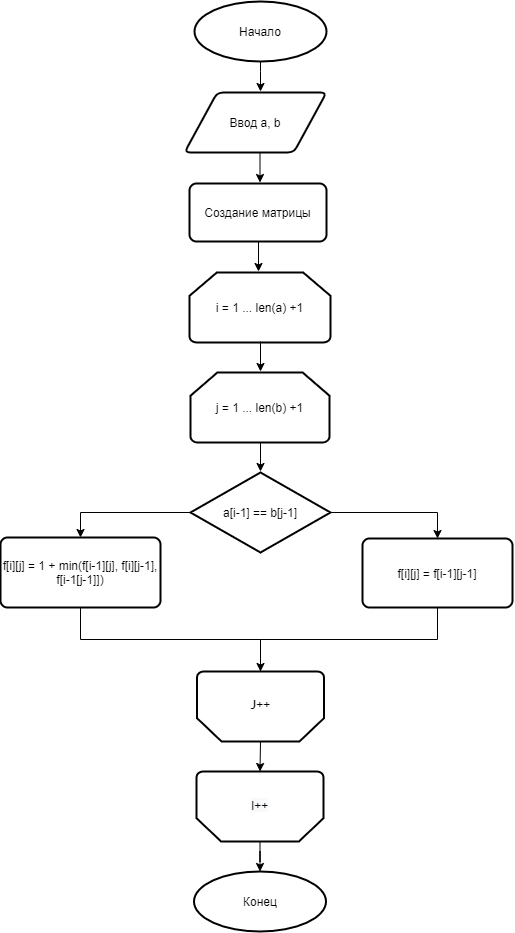
\includegraphics[width=12cm, height= 17cm]{diaglev.png}
	\captionsetup{justification=centering}
	\caption{Схема матричного алгоритма нахождения расстояния Левенштейна.}
	\label{Рис 1}
\end{figure}

\begin{figure}[H]
	\centering
	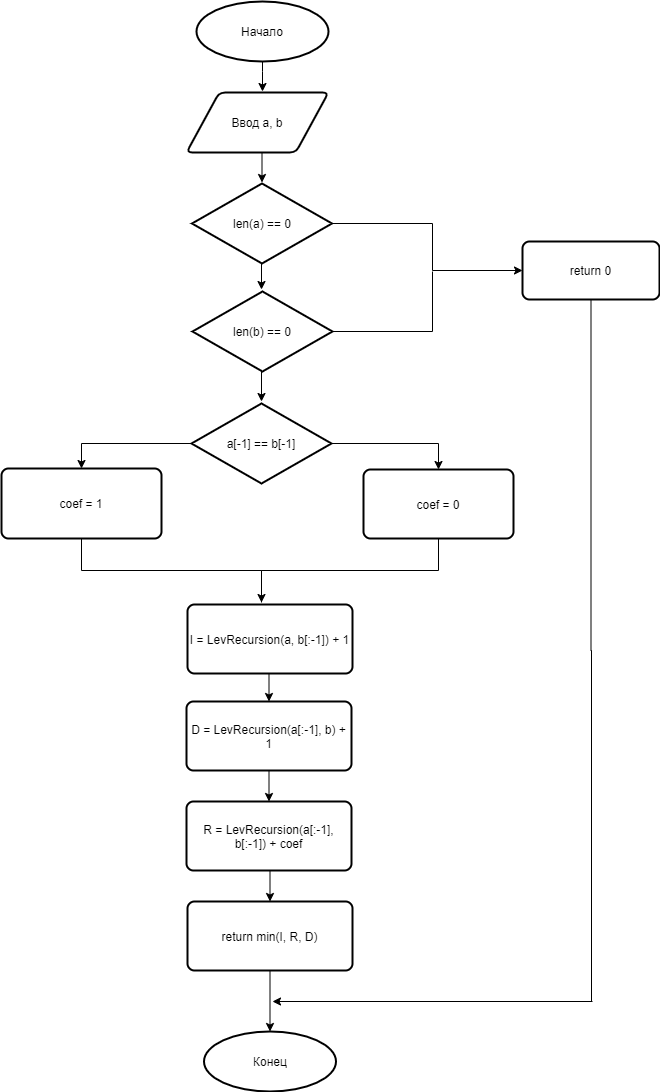
\includegraphics[width=12cm, height= 19cm]{levrec.png}
	\captionsetup{justification=centering}
	\caption{Схема рекурсивного алгоритма нахождения расстояния Левенштейна.}
	\label{Рис 2}
\end{figure}

\begin{figure}[H]
	\centering
	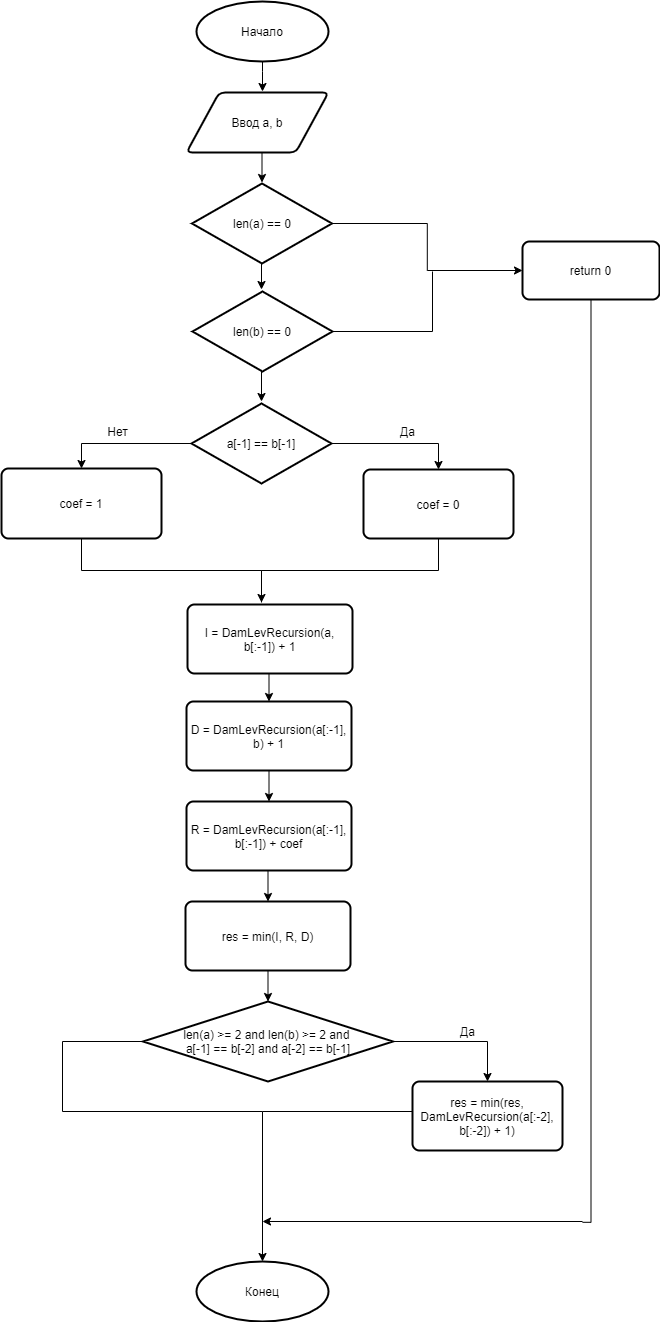
\includegraphics[width=12cm, height= 19cm]{damlevrec.png}
	\captionsetup{justification=centering}
	\caption{Схема рекурсивного алгоритма нахождения расстояния ДамерауЛевенштейна.}
	\label{Рис 3}
\end{figure}

\begin{figure}[H]
	\centering
	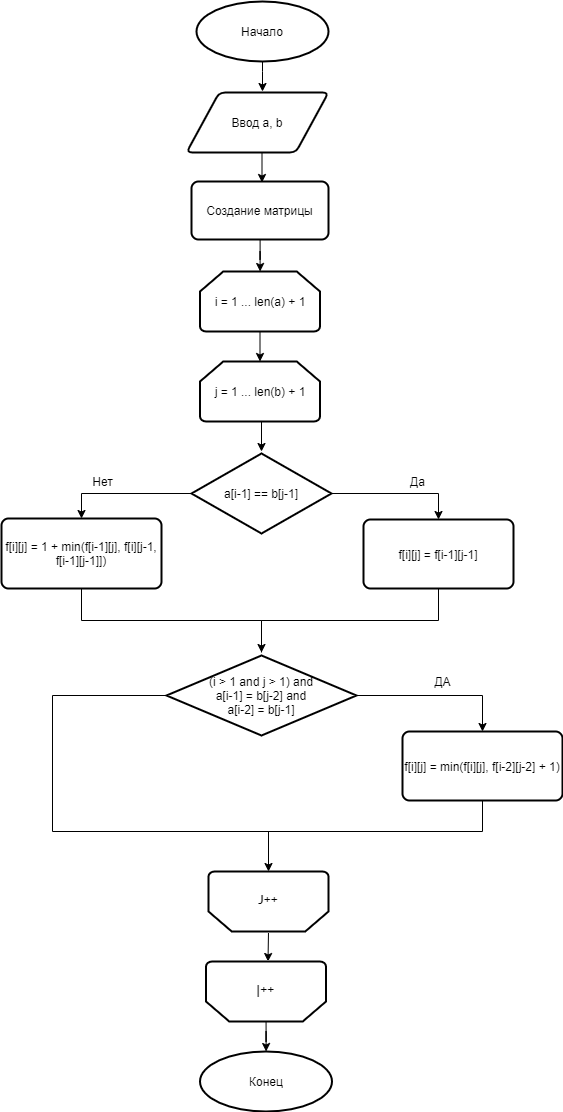
\includegraphics[width=12cm, height= 19cm]{damlevtable.png}
	\captionsetup{justification=centering}
	\caption{Схема матричного алгоритма нахождения расстояния ДамерауЛевенштейна}
	\label{Рис 4}
\end{figure}

\newpage
\section{Технологическая часть}

\hfill

В данном разделе будут рассмотрены требования к программному обеспечению, средства реализации и представлен листинг кода. 

\subsection{Требования к программному обеспечению}

\hfill

Программное обеспечение должно предоставлять возможность ввода двух строк (пустая строка считается корректным вводом), на выходе пользователь должен получить кратчайшее расстояние, вывод матрицы для всех алгоритмов, кроме Левенштейна с рекурсией. Также программное обеспечение должно обеспечить вывод замеров времени работы каждого из алгоритма.

\subsection{Средства реализации}

\hfill

В данной работе используется язык программирования Python, так как ЯП позволяет написать программу за кратчайшее время.В качестве среды разработки выбрана IDLE.
Для замеров времени была выбран метод process\_time() модуля time, он возвращает значение (в долях секунды) системного процессорного времени текущего процесса.

\subsection{Листинг кода}

В листингах 3.1 - 3.4 представлена реализация алгоритмов Левенштейна и Дамерау-Левенштейна.
\lstset{ %
	language=Python,                % Язык программирования 
	numbers=left,                   % С какой стороны нумеровать                           
}
 \textbf{\\Листинг 3.1 -- Расстояние Левинштейна }

\begin{lstlisting}
def levinstein(a, b):
	m = [[i+j if i*j == 0 else 0 for j in range(len(b) + 1)] 
					for i in range (len(a) + 1)]
	for i in range(1, len(a) + 1):
		for j in range (1, len(b) + 1):
			if a[i-1] == b[j-1]:
				m[i][j] = m[i-1][j-1]
			else:
				m[i][j] = 1 + min(m[i-1][j], m[i][j-1]
				                          , m[i-1][j-1])
	return m[len(a)][len(b)]
\end{lstlisting}
 \textbf{\\Листинг 3.2 -- Рекурсивное расстояние Левенштейна }

\begin{lstlisting}
def levinstein_recursive(a, b):
	if a ==  "" or b == "": 
		return abs(len(a) - len(b))
	coef = 0 if (a[-1] == b[-1]) else 1
	return min(levinstein_recursive(a, b[:-1]) + 1,
			   levinstein_recursive(a[:-1], b) + 1,
	           levinstein_recursive(a[:-1], b[:-1]) + coef)
\end{lstlisting}

 \textbf{\\Листинг 3.3 -- Расстояние Дамерау-Левенштейна }

\begin{lstlisting}
def damerau_levinstein(a, b):
	m = [[i+j if i*j == 0 else 0 for j in range(len(b) + 1)] 
						for i in range (len(a) + 1)]
	for i in range(1, len(a) + 1):
		for j in range(1, len(b) + 1):
		if a[i-1] == b[j-1]:
			m[i][j] = m[i-1][j-1]
		else:
			m[i][j] = 1 + min(m[i-1][j], m[i][j-1], m[i-1][j-1])
		if (i > 1 and j > 1) and a[i-1] == b[j-2] 
		                      and a[i-2] == b[j-1]:
			m[i][j] = min(m[i][j], m[i-2][j-2] + 1)
	return m[len(a)][len(b)]
\end{lstlisting}

 \textbf{\\Листинг 3.4 -- Рекурсивное расстояние Дамерау-Левенштейна }

\begin{lstlisting}
def damerau_lev_recursion(a, b):
	if a ==  "" or b == "":
		return abs(len(a) - len(b))
	coef = 0 if (a[-1] == b[-1]) else 1
	res = min(damerau_lev_recursion(a, b[:-1]) + 1,
			  damerau_lev_recursion(a[:-1], b) + 1,
			  damerau_lev_recursion(a[:-1], b[:-1]) + coef)
	if (len(a) >= 2 and len(b) >= 2 and a[-1] == b[-2] and a[-2] == b[-1]):
		res = min(res, damerau_lev_recursion(a[:-2], b[:-2]) + 1)
	return res
\end{lstlisting}

\subsection{Тестирование}
\hfill

На рисунке 5 показаны результаты тестирования. Колонки A и B - заранее приготовленные данные.
\begin{figure}[H]
	\centering
	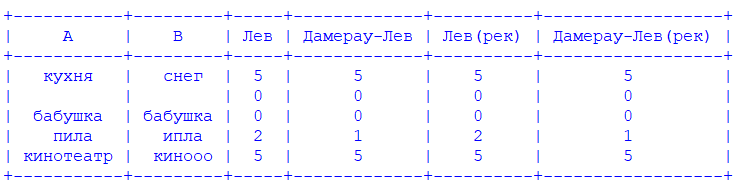
\includegraphics[scale=0.6]{test.png} 
	\captionsetup{justification=centering}
	\caption{Результаты работы программы на тестовых данных}
	\label{пример1}
\end{figure}

\subsection{Выводы}
В данном разделе была представлена реализация алгоритмов нахождения расстояния Левенштейна, Дамерау-Левенштейна, а также рекурсивные алгоритмы Левенштейна и Дамерау-Левенштейна. Программа корректно сработала на ввод пустых строк и строк, содержащих одинаковые символы, а так же при выполнении операций удаления, добавления, замены и транспозиции.
\newpage
\section{Экспериментальная часть}
\hfill

В данной части производится экспериментальное сравнение работы четырех реализованных алгоритмов (зависимость времени выполнения от длины входных слов).
\subsection{Постановка эксперимента}
\hfill

В рамках данной лабораторной работы были проведены следующие эксперименты:
\begin{enumerate} 
	\item Сравнение алгоритмов Левенштейна и Дамерау-Левенштейна. Количество символов в слове от 0 до 800 с шагом 50;
	
	\item Сравнение рекурсивного Левенштейна, матричного Левенштейна и рекурсивного Дамерау-Левенштейна. Количество символов в слове от 1 до 10 с шагом 2;
	
\end{enumerate} 
\subsection{Сравнительный анализ на материале экспериментальных данных}
\hfill

На рисунке 6 можно увидеть сравнение времени работы алгоритмов Левенштейна и Дамерау-Левенштейна.
\begin{figure}[H]
	\centering
	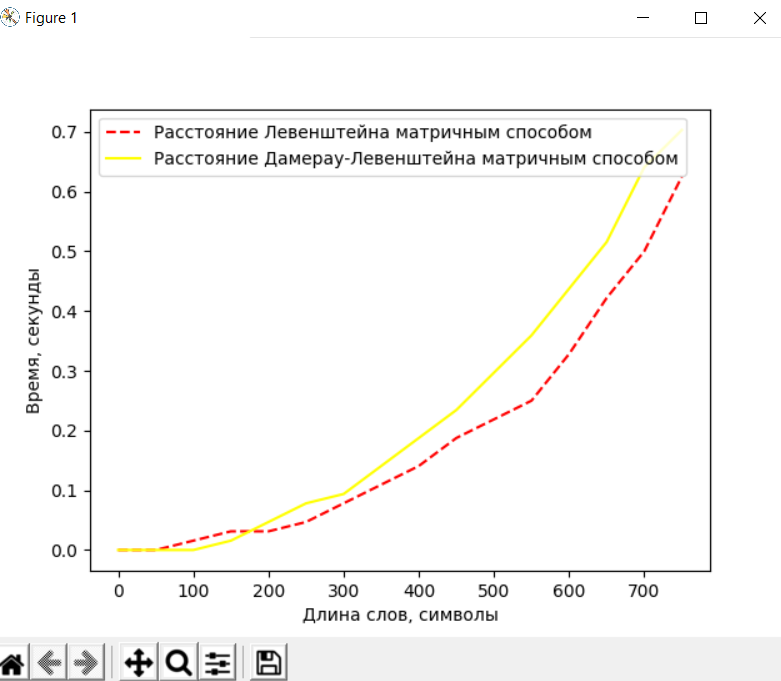
\includegraphics[scale=0.6]{exp1.png} 
	\captionsetup{justification=centering}
	\caption{График работы алгоритмов Левенштейна и Дамерау-Левенштейна}
	\label{эксперимент1}
\end{figure}
На рисунке 7 сравнение времени работы рекурсивных алгоритмов Левенштейна и Дамерау-Левенштейна.
\begin{figure}[H]
	\centering
	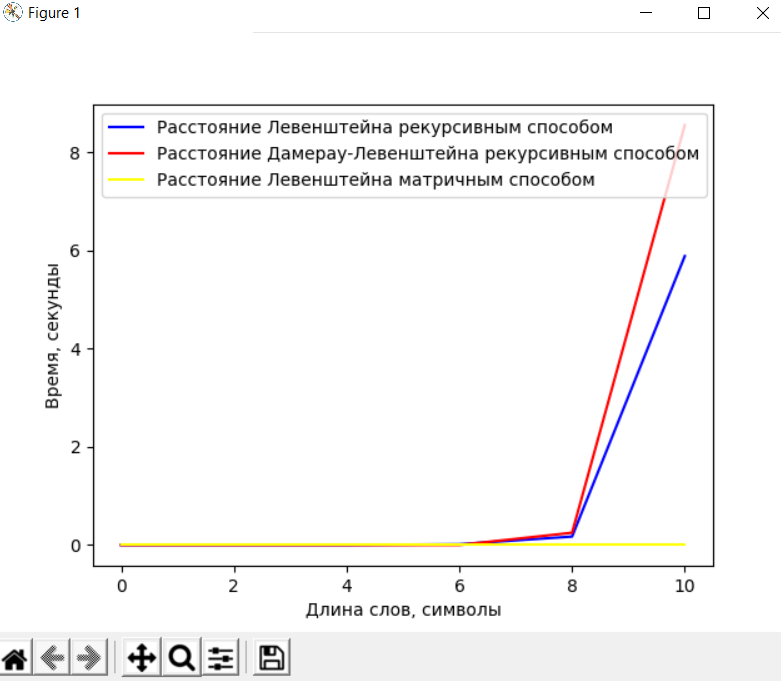
\includegraphics[scale=0.6]{exp2.png} 
	\captionsetup{justification=centering}
	\caption{График работы рекурсивных алгоритмов Левенштейна и Дамерау-Левенштейна, и матричного алгоритма Левенштейна}
	\label{эксперимент2}
\end{figure}
\subsection{Выводы}
В результате проведенного эксперимента был получен следующий вывод: рекурсивный алгоритм Левенштейна работает намного медленнее матричной реализации. Алгоритм Дамерау-Левенштейна незначительно проигрывает во времени алгоритму Левенштейна, это связано с дополнительными операциями, выполняющимися в ходе работы алгоритма. При сравнении графиков работы рекурсивных алгоритмой Левенштейна и Дамерау-Левенштейна можно заметить, что оба алгоритмы имеют одинаковый характер, но по скорости рекурсивный алгоритм Левенштейна работает быстрее, чем рекурсивный алгоритм Дамерау-Левенштейна.
\newpage
\anonsection{Заключение}
\hfill

В ходе работы были изучены алгоритмы нахождения расстояния Левенштейна и Дамерау-Левенштейна (рекурсивный и матричный). Выполнено сравнение рекурсивного и матричного алгоритмов ДамерауЛевенштейна.
При сравнении данных алгоритмов пришли к выводу, что рекурсивный алгоритм является самым медленным, поэтому по времени намного эффективнее использовать матричные алгоритмы.
\end{document} % Конец текста.

